\section{Crysis 2}

\begin{figure}[htbp]
\begin{center}
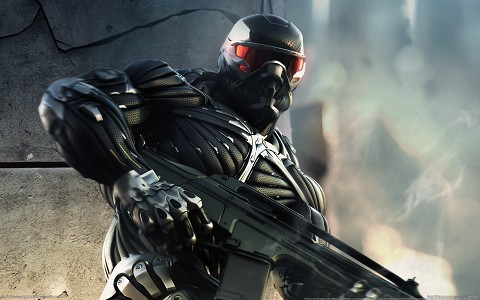
\includegraphics[width=.60\textwidth]{./imagenes/crysis2.jpg}
\caption{Crysis 2}
\label{Crysis 2}
\end{center}
\end{figure}
Crysis 2 \footnote{\url{http://www.ea.com/es/crysis2}} es un videojuego de disparos en primera persona desarrollado por la empresa Crytek y distribuido por Electronic Arts. Fue publicado en marzo de 2011 para PC, Xbox 360 y PlayStation 3. Es la secuela de Crysis y el primer videojuego en usar el motor CryEngine 3 desarrollado por Crytek también.

\subsubsection{¿Por qué es uno de mis juegos favoritos?}
\begin{itemize}
\item[Rubén Carvajal] La esencia del juego es magnifica, la historia consigue atraparte con su argumento futurístico.
Uno puede jugarlo a su manera, dependiendo del escenario habrán momentos en que te guste más pasar a todos descargando todo tu arcenal de armas, o momentos en que lo que sirva más sea utilizar las multiples opciones del traje y el sigilo.
La jugabilidad y los gráficos son de altísima calidad, las opciones de camuflaje y el entorno en el que se desarrolla el juego son particularidades destacables.

El sonido de cada ambiente está bien trabajado, e incluso tenemos opciones gráficas en 3D, cosas que hacen de este un exelente juego.
\end{itemize}